% Created 2012-10-15 lun. 14:49
\documentclass[smallextended]{svjour3}
\smartqed 
\usepackage[utf8]{inputenc}
\usepackage[T1]{fontenc}
\usepackage{fixltx2e}
\usepackage{graphicx}
\usepackage{longtable}
\usepackage{float}
\usepackage{wrapfig}
\usepackage{soul}
\usepackage{textcomp}
\usepackage{marvosym}
\usepackage[integrals]{wasysym}
\usepackage{latexsym}
\usepackage{amssymb}
\usepackage{hyperref}
\usepackage{algorithm}
\usepackage{algorithmic}
\usepackage{subfigure}
\tolerance=1000
%\usepackage{amsmath}
%\usepackage{amsthm}
%\newtheorem{definition}{Definition}
%\newtheorem{theorem}{Theorem}
\newtheorem{cor}{Corollary}
\usepackage{dsfont}
\usepackage{mathtools}
\mathtoolsset{showonlyrefs=true}
\providecommand{\alert}[1]{\textbf{#1}}
\newcommand{\E}{\mathbf{E}}
\newcommand{\argmax}{\operatorname*{argmax}} %\operatorname* pour les op. pouvant admettre des limites...
\newcommand{\Card}{\operatorname*{Card}} %\operatorname* pour les op. pouvant admettre des limites...
\begin{document}
\title{A cascaded supervised learning approach to inverse reinforcement learning}
\author{Edouard Klein$^{1,2}$ \and Bilal Piot $^{2,3}$\and Matthieu Geist $^{2}$\and Olivier Pietquin$^{2,3}$}
\titlerunning{Cascading approach to IRL}
\institute{
 1. ABC Team\\
 LORIA-CNRS, France.\\
\and
2. Supélec\\
 IMS-MaLIS Research group, France\\
 \texttt{firstname.lastname@supelec.fr}\\
\and 
3. UMI 2958 (GeorgiaTech-CNRS)\\
France\\
}
\date{\today}


\maketitle

\begin{abstract}
  This paper considers the Inverse Reinforcement Learning (IRL) problem, that is inferring a reward function for which a demonstrated expert policy is optimal.
We propose to break the IRL problem down into two generic Supervised Learning steps: this is the Cascaded Supervised IRL (CSI) approach. A classification step that defines a score function is followed by a regression step providing a reward function.
A theoretical analysis shows that the demonstrated expert policy is near-optimal for the computed reward function.
Not needing to repeatedly solve a Markov Decision Process (MDP) and the ability to leverage existing techniques for classification and regression are two important advantages of the CSI approach. It is furthermore empirically demonstrated to work with only transitions sampled according to the expert policy, up to the use of some heuristics. This is exemplified on two classical benchmarks (the mountain car problem and a highway driving simulator).
  \end{abstract}
\section{Introduction}
\label{sec-2}
Sequential decision making consists in choosing the appropriate action given the available data in order to maximize a certain criterion. When framed in a Markov Decision Process (MDP) (see Sec.~\ref{sec:background}), (Approximate) Dynamic programming ((A)DP) or Reinforcement Learning (RL) are often used to solve the problem by maximizing the expected sum of discounted rewards. The Inverse Reinforcement Learning (IRL)~\cite{russell1998learning} problem, which is addressed here, aims at inferring a reward function for which a demonstrated expert policy is optimal.

IRL is one of many ways to perform Apprenticeship Learning (AL): imitating a demonstrated expert policy, without necessarily explicitely looking for the reward function. The reward function nevertheless is of interest in its own right. As mentionned in \cite{russell1998learning}, its semantics can be analyzed in biology or econometrics for instance. Practically, the reward can be seen as a succinct description of a task. Discovering it removes the coupling that exists in AL between understanding the task and learning how to fulfill it. IRL allows the use of (A)DP or RL techniques to learn the task from the computed reward function. Although some approaches use it as a byproduct, most AL algorithm makes no use of the reward function, or have nothing to do with IRL altogether. A very straightforward non-IRL way to do AL is for example to use a multi-class classifier to directly learn the expert policy. We provide in the experiments (Sec.~\ref{sec:experiments}) a comparison between AL and IRL algorithms by using IRL as a way to do AL.

A lot of existing approaches in either IRL or IRL-based AL need to repeatedly solve the underlying MDP to find the optimal policies of intermediate reward functions. Thus, their performance depends strongly on the quality of the associated subroutine. Consequently, they suffer from the same challenges of scalability, data scarcity, etc., as RL and (A)DP. In order to avoid \emph{repeatedly} solving such problems, we adopt a different point of view.

Having in mind that there is a one to one relation between a reward function and its associated optimal action-value function (via the Bellman equation, see Eq.~\eqref{eq:bellman1}), it is worth thinking of a method able to output an action-value function for which the greedy policy is the demonstrated expert policy. Thus, the demonstrated expert policy will be optimal for the corresponding reward function. We propose to use a score function-based multi-class classification step (see Sec.~\ref{sec:algo}) to infer a score function. Besides, in order to retrieve via the Bellman equation the reward associated with the score function computed by the classification step, we introduce a regression step (see Sec.~\ref{sec:algo}). That is why the method is called the Cascaded Supervised Inverse reinforcement learning (CSI). This method is analyzed in Sec.~\ref{sec:analysis}, where it is shown that the demonstrated expert policy is near-optimal for the reward the regression step outputs.

This algorithm does not need to iteratively solve an MDP and requires only sampled transitions from expert and non-expert policies as inputs. Moreover, up to the use of some heuristics (see Sec.~\ref{subsubsec:heuristics}), the algorithm is able to be trained only with transitions sampled from the demonstrated expert policy. A specific instantiation of CSI (proposed Sec.~\ref{subsubsec:subroutines}) is tested on the mountain car problem (Sec.~\ref{subsec:mountaincar}) and on a highway driving simulator (Sec.~\ref{subsec:highway}) where we compare it with a pure classification algorithm \cite{taskar2005learning} and with two recent successfull IRL methods \cite{klein2012scirl} as well as with a random baseline.

Differences and similarities with existing AL or IRL approaches are succinctly discussed in Sec.~\ref{sec:related}.
\section{Background and notations}
\label{sec:background}
First, we introduce some general notations.
Let $E$ and $F$ be two non-empty sets, $E^F$ is the set of functions from $F$ to $E$.
We note $\Delta_X$ the set of distributions over $X$.
Let $\alpha\in\mathbb{R}^X$ and $\beta\in\mathbb{R}^X$: $\alpha\geq\beta \Leftrightarrow \forall x\in X, \alpha(x) \geq \beta(x)$. We will often slightly abuse the notations and consider (where applicable) most objects as if they were matrices and vectors indexed by the set they operate upon.

We work with finite MDPs \cite{puterman1994markov}, that is tuples $\{S,A,P,R,\gamma\}$. The state space is noted $S$, $A$ is a finite action space, $R\in\mathbb{R}^{S\times A}$ is a reward-function, $\gamma\in (0,1)$ is a discount factor and $P\in \Delta_{S}^{S\times A}$ is the Markovian dynamics of the MDP. Thus, for each $(s,a)\in S\times A$, $P(.|s,a)$ is a distribution over $S$ and $P(s'|s,a)$ is the probability to reach $s'$ by choosing action $a$ in state $s$. At each time step $t$, the agent uses the information encoded in the state $s_t\in S$ in order to choose an action $a_t \in A$ according to a (deterministic\footnote{We restrict ourselves here to deterministic policies, but the loss of generality is minimal as there exists at least one optimal deterministic policy.}) policy $\pi\in A^S$. The agent then steps to a new state $s_{t+1}\in S$ according to the Markovian transition probabilities $P(s_{t+1}|s_t,a_t)$. Given that $P_\pi = (P(s'|s,\pi(s)))_{s,s' \in S}$ is the irreductible transition probability matrix, the stationary distribution over the states $\rho_\pi$ induced by a policy $\pi$ satisfies
\begin{equation}
  \rho_\pi^TP_\pi = \rho_\pi^T\textrm{, with }X^T\textrm{ being the transpose of }X.
  \end{equation}
The stationary distribution relative to the exert policy $\pi_E$ is $\rho_E$.

The reward function $R$ is a local measure of the quality of the control. The global quality of the control induced by a policy $\pi$, with respect to a reward $R$, is assessed by the value function $V^\pi_R \in \mathbb{R}^{S}$ which associates to each state the expected discounted cumulative reward for following policy $\pi$ from this state:
\begin{equation}
V^\pi_R(s) = \E[\sum_{t\geq 0}\gamma^tR(s_t,\pi(s_t))|s_0 = s,\pi].
\end{equation}
This long-term criterion is what is being optimized when solving an MDP. Therefore, an optimal policy $\pi^*_R$ is a policy whose value function (the optimal value function $V^*_R$) is greater than that of any other policy, for all states: $\forall \pi, V^*_R\geq V^\pi_R$.

The Bellman evaluation operator $T^\pi_R: \mathbb{R}^{S} \rightarrow  \mathbb{R}^{S}$ is defined by
\begin{equation}
  T^{\pi}_RV = R_\pi + \gamma P_\pi V
  \end{equation}
where $R_\pi = (R(s,\pi(s)))_{s\in S}$. The Bellman optimality operator follows naturally:
\begin{equation}
  T^*_RV = \max_\pi T^\pi_RV.
\end{equation}
  Both operators are contractions. The fixed point of the Bellman evaluation operator $T^\pi_R$ is the value function of $\pi$ with respect to reward R:
  \begin{eqnarray}
    V^\pi_R &=& T^\pi_R V^\pi_R \Leftrightarrow V^\pi_R = R_\pi + \gamma P_\pi V^\pi_R.
  \end{eqnarray}
The Bellman optimality operator $T^*_R$ also admits a fixed point, the optimal value function $V_R^*$ with respect to reward $R$.

Another object of interest is the action-value function $Q^\pi_R\in\mathbb{R}^{S\times A}$ that adds a degree of freedom on the choice of the first action, formally defined by $Q^\pi_R(s,a) = T^a_RV^\pi_R(s)$, with $a$ the policy that always returns action $a$ ($T^a_RV = R_a + \gamma P_a V$ with $P_a = (P(s'|s,a))_{s,s' \in S}$ and $R_a$ = $(R(s,a))_{s\in S}$). The value function $V^\pi_R$ and the action-value function $Q^\pi_R$ are quite directly related: $\forall s \in S, V^\pi_R(s) = Q^\pi_R(s,\pi(s))$. The Bellman evaluation equation for $Q^\pi_R$ is therefore:
\begin{equation}
  Q^\pi_R(s,a) = R(s,a) + \gamma \sum_{s'\in S}P(s'|s,a) Q(s',\pi(s')).
  \label{eq:bellman1}
\end{equation}

An optimal policy follows a greedy mechanism with respect to its optimal action-value function $Q^*_R$:
\begin{equation}
  \label{eq:greedy}
  \pi^*_R(s)\in\argmax_aQ^*_R(s,a).
\end{equation}

When the state space is too large to allow matrix representations or when the transition probabilites or even the reward function are unknown except through observations gained by interacting with the system, RL or ADP may be used to approximate the optimal control policy~\cite{sutton1998reinforcement}.

We recall that solving the MDP is the direct problem. This contribution aims at solving the inverse one. We observe trajectories drawn from an expert's deterministic\footnotemark[\value{footnote}] policy $\pi_E$, assuming that there exists some unknown reward $R_E$ for which the expert is optimal. The suboptimality of the expert is an interesting setting that has been discussed for example in \cite{melo2010analysis,syed2010reduction}, but that we are not addressing here. We do not try to find this unknown reward $R_E$ but rather a non trivial reward $R$ for which the expert is at least near-optimal. The trivial reward $0$ is a solution to this ill-posed problem (no reward means that every behavior is optimal). Because of its ill-posed nature, this expression of \emph{Inverse Reinforcement Learning} (IRL) still has to find a satisfactory solution although a lot of progress has been made, see Sec.~\ref{sec:related}.
\section{The cascading algorithm}
\label{sec:algo}
Our first step towards a reward function solving the IRL problem is a classification step using a \emph{score function-based multi-class classifier} (SFMC$^2$ for short). This classifier learns a score function $q\in\mathbb{R}^{S\times A}$ that rates the association of a given action\footnote{Here, actions play the role of what is known as {\it labels} or {\it categories} when talking about classifiers.} $a\in A$ with a certain input $s\in S$. The classification rule $\pi_C\in A^S$ simply selects (one of) the action(s) that achieves the highest score for the given inputs:
\begin{equation}
  \label{eq:greedy2}
\pi_C(s) \in \argmax_a q(s,a).
\end{equation}
For example, \emph{Multi-class Support Vector Machines}~\cite{guermeur2011generic} can be seen as SFMC$^2$ algorithms, the same can be said of the structured margin approach \cite{taskar2005learning} both of which we consider in the experimental setting. Other algorithms may be envisionned (see Sec.~\ref{subsubsec:subroutines}). 

Given a dataset $D_C = \{(s_i,a_i=\pi_E(s_i))_i\}$ of actions $a_i$ (deterministically) chosen by the expert on states $s_i$, we train such a classifier. The classification policy $\pi_C$ is not the end product we are looking for (that would be mere supervised imitation of the expert, not IRL). What is of particular interest to us is the score function $q$ itself. One can easily notice the similarity between Eq.~\eqref{eq:greedy2} and Eq.~\eqref{eq:greedy} that describes the relation between the optimal policy in an MDP and its optimal action-value function. The score function $q$ of the classifier can thus be viewed as some kind of optimal action-value function for the classifier policy $\pi_C$. By inversing the Bellman equation \eqref{eq:bellman1} with $q$ in lieu of $Q^\pi_R$, one gets $R^C$, the reward function relative to our score/action-value function $q$:
\begin{equation}
  \label{eq:rc}
  R^C(s,a) =q(s,a) - \sum_{\mathrm{s'}}P(s'|s,a)q(s',\pi_C(s')).
\end{equation}
As we wish to approximately solve the general IRL problem where the transition probabilities $P$ are unknown, our reward function $R^C$ will be approximated with the help of information gathered by interacting with the system. We assume that another dataset $D_R = \{(s_j,a_j,s'_j)_j\}$ is available where $s'_j$ is the state an agent taking action $a_j$ in state $s_j$ transitioned to. Action $a_j$ need not be chosen by any particular policy. The dataset $D_R$ brings us information about the dynamics of the system. From it, we construct datapoints
\begin{equation}
  \label{eq:rj}
  \{\hat r_j = q(s_j,a_j) - \gamma q(s'_j,\pi_C(s'_j))\}_j.
\end{equation}
As $s'_j$ is sampled accordingly to $P(\cdot|s_j,a_j)$ the constructed datapoints help building a good approximation of $R^C(s_j,a_j)$. A regressor (a simple least-square approximator can do but other solutions could also be envisionned, see Sec.~\ref{subsubsec:subroutines}) is then fed the datapoints $((s_j,a_i),\hat r_j)$ to obtain $\hat R^C$, a generalisation of $\{((s_j,a_j),\hat r_j)_j\}$ over the whole state-action space. The complete algorithm is given in Alg.~\ref{algo:cascading}.

There is no particular constraint on $D_C$ and $D_R$. Clearly, there is a direct link between various qualities of those two sets (amount of data, statistical representativity, etc.) and the classification and regression errors. The exact nature of the relationship between these quantities depends on which classifier and regressor are chosen. The theoretical analysis of Sec.~\ref{sec:analysis} abstracts itself from the choice of a regressor and a classifier and from the composition of $D_C$ and $D_R$ by reasoning with the classification and regression errors. In Sec.~\ref{sec:experiments}, %FIXME subsec heuristic
the use of a single dataset to create both $D_C$ and $D_R$ is thoroughly explored.
\begin{algorithm}%[H]
    %\small
  \caption{CSI algorithm}
  \label{algo:cascading}
  \emph{\textbf{Given}} a training set $D_C=\{(s_i,a_i=\pi_E(s_i))\}_{1\leq i \leq D}$ and another training set $D_R=\{(s_{j},a_{j},s'_{j})\}_{1\leq j \leq D'}$\;\\
  \emph{\textbf{Train}} a score function-based classifier on $D_C$, obtaining decision rule $\pi_C$ and score function $q:S\times A \rightarrow \mathbb R$\;\\
  \emph{\textbf{Learn}} a reward function $\hat R^C$ from the dataset $\{((s_{j},a_{j}),\hat{r}_j)\}_{1\leq j \leq D'}$, $\forall (s_j,a_j,s'_j) \in D_R,\hat{r}_j=q(s_{j},a_{j})-\gamma q(s'_{j},\pi_C(s'_{j}))$\;\\
  \emph{\textbf{Output}} the reward function $\hat R^{C}$ \;
\end{algorithm}

Cascading two supervised approaches like we do is a way to inject the MDP structure into the resolution of the problem. Indeed, mere classification only takes into account information from the expert (i.e., which action goes with which state) whereas using the Bellman equation in the expression of $\hat r_j$ makes use of the information lying in the transitions $(s_j,a_j,s'_j)$, namely information about the transition probabilities $P$. The final regression step is a way to generalize this information about $P$ to the whole state-action space in order to have a well-behaved reward function.

Being able to alleviate the ill effects of scalability or data scarcity by leveraging the wide range of techniques developped for the classification and regression problems is a strong advantage of the CSI approach.

\section{Analysis}
\label{sec:analysis}


In this section, we prove that the deterministic expert policy $\pi_E$ is near optimal for the reward $\hat{R}^C$ the regression step outputs.
More formally, recalling from Sec.~\ref{sec:background} that $\rho_E$ is the stationary distribution of the expert policy, we prove that $\E_{s\sim\rho_E}[V^*_{\hat{R}^C}(s)-V^{\pi_E}_{\hat{R}^C}(s)]$ is bounded by a term that depends on:
\begin{itemize}
  \item the classification error defined as
\begin{equation}  
\epsilon_C=\E_{s\sim\rho_E}[\mathds{1}_{\{\pi_C(s)\neq\pi_E(s)\}}];
\end{equation}
\item the regression error defined as 
  \begin{equation}
    \epsilon_R=\max_{\pi\in A^S}\|\epsilon_\pi^R\|_{1,\rho_E},
  \end{equation}
  with:
  \begin{itemize}
  \item the subscript notation already used for $R_\pi$ and $P_\pi$ in Sec.~\ref{sec:background} meaning that, given an $X\in\mathbb{R}^{S\times A}$, $\pi\in A^S$, and $a\in A$,  $X_\pi\in\mathbb{R}^S$ and $X_a\in\mathbb{R}^S$ are respectively such that: $\forall s\in S, X_\pi(s)=X(s,\pi(s))$ and $\forall s\in S, X_a(s)=X(s,a)$ ;
  \item $\epsilon^R_\pi=R^C_\pi-\hat{R}^C_\pi$ ;
  \item $\|.\|_{1,\mu}$ the $\mu$-weighted $L_1$ norm: $\|f\|_{1,\mu} = \E_{x\sim \mu}[|f(x)|]$;
  \end{itemize}
\item the concentration coefficient $C_* = C_{\hat \pi_C}$ with:
  \begin{itemize}
  \item $C_{\pi}=(1-\gamma)\sum_{t\geq0}\gamma^tc_{\pi}(t), \text{ with } c_{\pi}(t)=\max_{s\in S}\frac{(\rho_E^TP^t_\pi)(s)}{\rho_E(s)}$ ;
  \item $\hat \pi_C$, the optimal policy for the reward $\hat R^C$ output by the algorithm ;
  \end{itemize}
  The constant $C_*$ can be estimated \emph{a posteriori} (after $\hat{R}^C$ is computed). {\it A priori}, $C_*$ can be upper-bounded by a more usual and general concentration coefficient but $C_*$ gives a tighter final result: one can informally see $C_*$ as a measure of the similarity between the distributions induced by $\hat\pi_C$ and $\pi_E$ (roughly, if $\hat{\pi}_C\approx\pi_E$ then $C_* \approx 1$).
\item $\Delta q$, defined by 
  \begin{eqnarray}
    \Delta q &= &\max_{s\in S}(\max_{a\in A}q(s,a)-\min_{a\in A}q(s,a))=\max_{s\in S}(q(s,\pi_C(s))-\min_{a\in A}q(s,a)),
    \end{eqnarray} which could be normalized to $1$ without loss of generality. The range of variation of $q$ induces the one of $R^C$, $\hat{R}^C$ and $V^{\pi_C}_{\hat{R^C}}$.
  \end{itemize}
\begin{theorem}
\label{thm}
Let $\pi_E$ be the deterministic expert policy, $\rho_E$ its stationary distribution and $\hat{R}^C$ the reward the cascading algorithm outputs. We have:
\begin{equation}
0\leq\E_{s\sim\rho_E}[V^*_{\hat{R}^C}(s)-V^{\pi_E}_{\hat{R}^C}(s)]\leq \frac{1}{1-\gamma}\left(\epsilon_C\Delta q +\epsilon_R(1+C_*)\right).
\end{equation}
\end{theorem}
\begin{proof}
First let's recall some notations, $q\in\mathbb{R}^{S\times A}$ is the score function output by the classification step, $\pi_C$ is a deterministic classifier policy so that $\forall s \in S,\pi_C(s)\in\argmax_{a\in A}q(s,a)$, $R^C\in\mathbb{R}^{S\times A}$ is:
\begin{equation}
\forall (s,a)\in S\times A, R^C(s,a)=q(s,a) -\gamma\sum_{s'\in S}P(s'|s,a)q(s',\pi_C(s')),
\end{equation}
and $\hat{R}^C\in\mathbb{R}^{S\times A}$ is the reward function output by the regression step.

The difference between $R^C$ and $\hat{R}^C$ is noted $\epsilon^R=R^C-\hat{R}^C$.
We also introduce the reward function $R^E\in\mathbb{R}^{S\times A}$ which will be useful in our proof, not to be confused with $R_E$ the unknown reward function the expert optimizes:
\begin{equation}
\forall (s,a)\in S\times A, R^E(s,a)=q(s,a) -\gamma\sum_{s'\in S}P(s'|s,a)q(s',\pi_E(s')).
\end{equation}

We can now introduce the following vectorial equations:
\begin{align}
&R^C_a=q_a-\gamma P_aq_{\pi_C},
\\
&R^E_a=q_a-\gamma P_aq_{\pi_E},
\\
&\epsilon^R_a=R^C_a-\hat{R}^C_a.
\end{align}
Now, we are going to upper bound the term: $\E_{s\sim\rho_E}[V^*_{\hat{R}^C}-V^{\pi_E}_{\hat{R}^C}]\geq0$ (the lower bound is obvious as $V^*$ is optimal).
Recall that $\hat{\pi}_C$ is a deterministic optimal policy of the reward $\hat{R}^C$. First, the term $V^*_{\hat{R}^C}-V^{\pi_E}_{\hat{R}^C}$ is decomposed:
\begin{equation}
V^*_{\hat{R}^C}-V^{\pi_E}_{\hat{R}^C}=(V^{\hat{\pi}_C}_{\hat{R}^C}-V^{\hat{\pi}_C}_{R^C})+(V^{\hat{\pi}_C}_{R^C}-V^{\pi_E}_{R^C})+(V^{\pi_E}_{R^C}-V^{\pi_E}_{\hat{R}^C}).
\end{equation}
We are going to bound each of these three terms. First, let $\pi$ be a given deterministic policy. We have, using $\epsilon^R = R^C - \hat R^C$:
\begin{equation}
V^{\pi}_{R^C}-V^{\pi}_{\hat{R}^C}=V^{\pi}_{\epsilon^R}=(I-\gamma P_\pi)^{-1}\epsilon^R_{\pi}.
\end{equation}
If $\pi=\pi_E$, we have, thanks to the power series expression of $(I-\gamma P_{\pi_E})^{-1}$, the definition of $\rho_E$ and the definition of the $\mu$-weighted $L_1$ norm, one property of which is that $\forall X, \mu^TX \leq \|X\|_{1,\mu}$:
\begin{equation}
  \rho_E^T(V^{\pi}_{R^C}-V^{\pi}_{\hat{R}^C})=\rho_E^T(I-\gamma P_{\pi_E})^{-1}\epsilon^R_{\pi_E}=\frac{1}{1-\gamma}\rho_E^T\epsilon^R_{\pi_E}\leq\frac{1}{1-\gamma}\|\epsilon^R_{\pi_E}\|_{1,\rho_E}.\end{equation}

If $\pi\neq\pi_E$, we use the concentration coefficient $C_\pi$. We have then:
\begin{equation}
  \rho_E^T(V^{\pi}_{R^C}-V^{\pi}_{\hat{R}^C})\leq\frac{C_\pi}{1-\gamma}\rho_E^T\epsilon^R_{\pi}\leq\frac{C_\pi}{1-\gamma}\|\epsilon^R_{\pi}\|_{1,\rho_E}.
  \end{equation}
So, using the notations introduced before we stated the theorem, we are able to give an upper bound to the first and third terms (recall also the notation $C_{\hat \pi_C} = C_*$):
\begin{equation}
\rho_E^T((V^{\pi_E}_{R^C}-V^{\pi_E}_{\hat{R}^C})+(V^{\hat{\pi}_C}_{\hat{R}^C}-V^{\hat{\pi}_C}_{R^C}))\leq\frac{1+C_*}{1-\gamma}\epsilon_R.
\end{equation}
Now, there is still an upper bound to find for the second term. It is possible to decompose it as follows:
\begin{equation}
V^{\hat{\pi}_C}_{R^C}-V^{\pi_E}_{R^C}=(V^{\hat{\pi}_C}_{R^C}-V^{\pi_C}_{R^C})+(V^{\pi_C}_{R^C}-V^{\pi_E}_{R^E})+(V^{\pi_E}_{R^E}-V^{\pi_E}_{R^C}).
\end{equation}
By construction, $\pi_C$ is optimal for $R^C$, so $V^{\hat{\pi}_C}_{R^C}-V^{\pi_C}_{R^C}\leq0$ which implies:
\begin{equation}
V^{\hat{\pi}_C}_{R^C}-V^{\pi_E}_{R^C}\leq(V^{\pi_C}_{R^C}-V^{\pi_E}_{R^E})+(V^{\pi_E}_{R^E}-V^{\pi_E}_{R^C}).
\end{equation}
By construction, we have $V^{\pi_C}_{R^C}=q_{\pi_C}$ and $V^{\pi_E}_{R^E}=q_{\pi_E}$, thus:
\begin{eqnarray}
\rho_E^T(V^{\pi_C}_{R^C}-V^{\pi_E}_{R^E})&=&\rho_E^T(q_{\pi_C}-q_{\pi_E})\\
&=&\sum_{s\in S}\rho_E(s)(q(s,\pi_C(s))-q(s,\pi_E(s)))[\mathds{1}_{\{\pi_C(s)\neq\pi_E(s)\}}].
\end{eqnarray}
Using $\Delta q$, we have:
\begin{equation}
\rho_E^T(V^{\pi_C}_{R^C}-V^{\pi_E}_{R^E})\leq\Delta q\sum_{s\in S}\rho_E(s)[\mathds{1}_{\{\pi_C(s)\neq\pi_E(s)\}}]= \Delta q \epsilon_C.
\end{equation}
Finally, we also have:
\begin{align}
\rho_E^T(V^{\pi_E}_{R^E}-V^{\pi_E}_{R^C})&=\rho_E^T(I-\gamma P_{\pi_E})^{-1}(R^E_{\pi_E}-R^C_{\pi_E}),
\\
&=\rho_E^T(I-\gamma P_{\pi_E})^{-1}\gamma P_{\pi_E}(q_{\pi_C}-q_{\pi_E}),
\\
&=\frac{\gamma}{1-\gamma}\rho_E^T(q_{\pi_C}-q_{\pi_E})\leq \frac{\gamma}{1-\gamma}\Delta q \epsilon_C \leq  \frac{1}{1-\gamma}\Delta q \epsilon_C\textrm{ as }\gamma<1.
\end{align}
So the upper bound for the second term is: $\rho_E^T(V^{\hat{\pi}_C}_{R^C}-V^{\pi_E}_{R^C})\leq \frac{\Delta q}{1-\gamma}\epsilon_C$.
If we combine all of the results, we obtain the final bound:
\begin{equation}
0\leq\E_{s\sim\rho_E}[V^*_{\hat{R}^C}(s)-V^{\pi_E}_{\hat{R}^C}(s)]\leq \frac{1}{1-\gamma}(\epsilon_C\Delta q +\epsilon_R(1+C_*))).
\end{equation}
\qed
\end{proof}
Readers familiar with the work presented in \cite{klein2012scirl} will see some similarities between the theoretical analyses of SCIRL and CSI as both study error propagation in IRL algorithms. Another shared feature is the use of the score function $q$ of the classifier as a proxy for the action-value function of the expert $Q^{\pi_E}_{R_E}$. \\
The attentive reader, however, will percieve that similarities stop there. The error terms occurring in the two bounds are not related to one another. As CSI makes no use of the feature expectation of the expert, what is known as $\bar\epsilon_Q$ in \cite{klein2012scirl} does not appear in this analysis. Likewise, the regression error $\epsilon_R$ of this paper does not appear in the analysis of SCIRL, which does not use a regressor. Perhaps more subtly, the classification error and classification policy known in both papers as $\epsilon_C$ and $\pi_C$ are not the same. The classification policy of SCIRL is no tantamount to what is called $\pi_C$ here. For SCIRL, $\pi_C$ is the greedy policy for an approximation of the value function of the expert with respect to the reward output by the algorithm. For CSI, $\pi_C$ is the decision rule of the classifier, an object that is not aware of the structure of the MDP. We shall also mention that the error terms appearing in the CSI bound are more standard than the ones of SCIRL ({\it e.g.}, regression error vs feature expectation estimation error) thus they may be easier to control.
A direct corollary of this theorem is that, given perfect classifier and regressor, CSI produces a reward function for which $\pi_E$ is the \emph{unique} optimal policy.
\begin{corollary}
  \label{cor}
  Assume that $\rho_E>0$ and that the classifier and the regressor are perfect ($\epsilon_C = 0$ and $\epsilon_R = 0$). Then $\pi_E$ is the \emph{unique} optimal policy for $\hat R^C$.
\end{corollary}
\begin{proof}

  The function $q$ is the optimal action-value function for $\pi_C$ with respect to the reward $R^C$, by definition (see Eq.~\eqref{eq:rc}).
  As $\epsilon_C = 0$, we have $\pi_C = \pi_E$. This means that $\forall s, \pi_E(s)$ is the only element of the set $\argmax_{a\in A}q(s,a)$. Therefore, $\pi_C = \pi_E$ is the unique optimal policy for $R^C$.
  As $\epsilon_R = 0$, we have $\hat R^C = R^C$, hence the result.
  \qed
\end{proof}
This corollary hints at the fact that we found a non-trivial reward (we recall that the null reward admits \emph{every} policy as optimal). Therefore, obtaining  $\hat{R}_C = 0$ (for which the bound is obviously true: the bounded term is $0$, the bounding term is positive) is unlikely as long as the classifier and the regressor exhibit decent performance.

The only constraints the bound of Th.~\ref{thm} implies on datasets $D_R$ and $D_C$ is that they provide enough information to the supervised algorithms to keep both error terms $\epsilon_C$ and $\epsilon_R$ low. In Sec.~\ref{sec:experiments} we deal with a lack of data in dataset $D_R$. We address the problem with the use of heuristics (Sec.~\ref{subsubsec:heuristics}) in order to show the behavior of the CSI algorithm in somewhat more realistic (but difficult) conditions.

More generally, the error terms  $\epsilon_C$ and $\epsilon_R$ can be reduced by a wise choice for the classification and regression algorithms. The litterature is wide enough for methods accomodating most of use cases (lack of data, fast computation, bias/variance trade-off, etc.) to be found. Being able to leverage such common algorithms as multi-class classifiers and regressors is a big advantage of our cascading approach over existing IRL algorithms.

Other differences between existing IRL or apprenticeship learning approaches and the proposed cascading algorithm are further examined Sec.~\ref{sec:related}.

%% Feel good comment
\section{Experiments}
\label{sec:experiments}
In this section, we empirically demonstrate the behavior of our approach. We begin by providing information pertaining to both benchmarks: an explanation about the amount and source of the available data, the rationale behind the heuristics we use to compensate for the dire data scarcity and a quick word about the contenders CSI is compared to are given Sec.~\ref{subsec:generalities}. We supply quantitative results and comparisons of CSI with state-of-the art approaches on first a classical RL benchmark (the mountain car) Sec.~\ref{subsec:mountaincar} and then on a more difficult highway driving simulator (Sec.~\ref{subsec:highway}).
\subsection{Generalities}
\label{subsec:generalities}
\subsubsection{Data scarcity}
\label{subsubsec:data}
The CSI algorithm was designed not to repeatedly solve the RL problem. This feature makes it particularly well-suited to environments where sampling the MDP is difficult or costly. In the experiments, CSI is fed only with data sampled according to the expert policy. This corresponds for example to a situation where a costly system can only be controlled by a trained operator as a bad control sequence could lead to a system breakdown.

More precisely, the expert controls the system for $M$ runs of lengths $\{L_i\}_{1\leq i \leq M}$, %with values of $n$ in $\{3,7,10,15,20\}$,
giving samples $\{(s_k,a_k=\pi_E(a_k),s'_k)_k\} = D_E$. The dataset $D_C$ fed to the classifier is straightforwardly constructed from $D_E$ by dropping the $s'_k$ terms:
\begin{equation}
  D_C = \{(s_i = s_k,a_i=a_k)_i\}.
\end{equation}
\subsubsection{Heuristics}
\label{subsubsec:heuristics}

There is no particular problem for the classification step. It is however not reasonable to construct the dataset $D_R = \{((s_k,a_k=\pi_E(s_k)),\hat r_k)_k\}$ only from expert transitions and expect a small regression error term $\epsilon_R$. Indeed, the dataset $D_E$ only samples the dynamics induced by the expert's policy and not the whole dynamics of the MDP. 
This means that for a certain state $s_k$ we only know the corresponding expert action $a_k=\pi_E(s_k)$ and the following state $s'_k$ sampled according to the MDP dynamics : $s'_k \sim P(\cdot|s_k,a_k)$. For the regression to be meaningful, we need samples associating the same state $s_k$ and a different action $a\neq a_k$ with a datapoint $\hat r \neq \hat r_k$.\\
Recall that $\hat r_j = q(s_j,a_j) - \gamma q(s'_j,\pi_C(s'_j))$ (Eq.~\eqref{eq:rj}); without knowing $s'_k \sim P(\cdot|s_k,a\neq a_k)$, we cannot provide the regressor with a datapoint to associate with $(s_k,a\neq a_k)$.
We artificially augment the dataset $D_R$ with samples $((s_j=s_k,a),r_{min})_{j;\forall a\neq \pi_E(s_j) = a_k}$ where
\begin{equation}
  r_{min} = \min_k\hat r_k - 1.
\end{equation}
This heuristics intructs the regressor to associate a state-action tuple disagreeing with the expert ({\it i.e.}, $(s_k,a\neq a_k)$) with a reward strictly inferior to any of those associated with expert state action tuples ({\it i.e.}, $(s_k,a_k=\pi_E(s_k))$). Semantically, we are asserting that disagreeing with the expert in states the expert visited is a bad idea. This heuristics says nothing about states absent from the expert dataset. For such states the generalization capabilities of the regressor and, later on, the exploration of the MDP by an agent optimizing the reward will solve the problem.
Although this heuristics was not analyzed in Sec.~\ref{sec:analysis} (where the availability of a more complete dataset $D_R$ was assumed), the results shown in the next two subsections demonstrate its soundness.
\subsubsection{Comparison with state-of-the-art approaches}
The similar looking yet fundamentally different algorithm SCIRL \cite{klein2012scirl} is an obvious choice as a contender to CSI as it advertises the same ability to work with very little data, without repeatedly solving the RL problem. In both experiments we give the exact same data to CSI and SCIRL.

The algorithm of \cite{dvijotham2010inverse} also advertises not having to solve the RL problem, but needs to deal with linearly solvable MDPs, therefore we do not include it in our tests. The Relative Entropy (RE) method of \cite{boularias2011relative} has no such need, so we included it in our benchmarks. It could not, however, work with the small amount of data we provided SCIRL and CSI with, so to allow for importance sampling, we created another dataset $D_{random}$ that was used by RE but not by SCIRL nor CSI.

Finally, the classification policy $\pi_C$ output by the classification step of CSI was evaluated as well. Comparing classification and IRL algorithms makes no sense if the object of interest is the reward itself as can be envisionned in a biological or economical context. It is however sound to do so in an imitation context where what matters is the performance of the agent with respect to some objective criterion. Both experiments use such a criterion. Classification algorithms don't have to optimize any reward, the classification policy can directly be used in the environment. IRL algorithms on the other hand output a reward that must then be plugged in an RL or DP algorithm to get a policy. In each benchmark we used the same (benchmark-dependant) algorithm to get a policy from each of the three rewards output by SCIRL, CSI and RE. It is these policies whose performance we show. Finding a policy from a reward is of course a non-trivial problem that should not be swept under the rug, nevertheless we choose not to concern ourselves with it here as we wish to focus on IRL algorithms, not RL or DP algorithms. In this regard, using a classifier that directly outputs a policy may seem a much simpler solution, but we hope that the reader will be convinced that the gap in performance between classification and IRL is worth the trouble of solving the RL problem (once and for all, and not repeatedly as a subroutine like some other IRL algorithms).

We do not compare CSI to other IRL algorithms requiring repeatedly solving the MDP: as we would need to provide them with enough data to do so, the comparison makes little sense.
\subsubsection{Supervised Steps}
\label{subsubsec:subroutines}
The cascading algorithm can be instanciated with some standard classification algorithms and any regression algorithm. The choice of such subroutines may be dictated by the kind and amount of available data, by ease of use or by computational complexity, for example.

We referred in Sec.\ref{sec:algo} to \emph{score-function based multi-class classifiers} and explained how the classification rule is similar to the greedy mechanism that exists between an optimal action-value function and an optimal policy in an MDP. Most classification algorithm can be seen as such a classifier. In a simple $k$-nearest neighboor approach, for example, the score function $q(s,a)$ is the number of elements of class $a$ among the $k$-nearest neighboors of $s$. The generic M-SVM model makes the score function explicit (see \cite{guermeur2011generic}) (we use a SVM in the mountain car experiment Sec.~\ref{subsec:mountaincar}). In the highway experiment, we choose to use a structured margin classification approach \cite{taskar2005learning}.
%% that, given a feature vector $\phi: S\times A \rightarrow \mathbb{R}^p$ solves:
%% \begin{eqnarray*}
%%   &\min_{\theta,\zeta}\frac{1}{2}\|\theta\|^2 +
%%   \frac{\eta}{N}\sum_{i=1}^N \zeta_i \\
%%   &\text{~s.t.~} \forall i,
%%   \theta^T{\phi}(s_i,a_i)+\zeta_i \geq \max_a \theta^T
%%   {\phi}(s_i,a) + l(s_i,a). \label{eq:qp_taskar}
%% \end{eqnarray*}
%% with $l(s_i,a) = 1\textrm{ if } a\neq a_i \textrm{ and } l(s_i,a_i)=0$. The score function of this classifier is simply $q(s,a) = \theta^T \phi(s,a)$.
We chose a SVR as a regressor in the mountain car experiment and a simple least-square regressor on the highway.
%% Using the same features $\phi$ as our classifier, we introduce $\lambda$ a regularization coefficient (set to $0.1$ in our experiments), $I$ the identity matrix and 
%% \begin{eqnarray}
%%   \Phi = \begin{bmatrix}
%%     \vdots\\
%%     \phi(s_j,a_j)\\
%%     \vdots
%%   \end{bmatrix} \in \mathbb{R}^{n|A|\times p}\textrm{ and }
%%   \hat R = \begin{bmatrix}
%%     \vdots\\
%%     \hat r_j\\
%%     \vdots
%%   \end{bmatrix}\in \mathbb{R}^{n|A|},
%% \end{eqnarray}
%% with $r_j = r_{min}$ if $a_j \neq \pi_E(s_j)$. Our regressor can be written:
%% \begin{equation}
%%   \omega = (\Phi^T\Phi + \lambda I)^{-1}\Phi^T\hat R.
%% \end{equation}
%% The reward function is: $\hat R^C(s,a) = \omega^T \phi(s,a)$

It is possible to get imaginative in the last step. For example, using a Gaussian process regressor \cite{rasmussen2006gaussian} that outputs both expectation and variance can enable (nonwithstanding a nontrivial amount of work) the use of reward-uncertain reinforcement learning \cite{regan2011robust}. 

Our complete instanciation of CSI is summed up in Alg.~\ref{alg:CSIimp}.
\begin{algorithm}%[H]
    %\small
  \caption{A CSI instanciation with heuristics}
  \label{alg:CSIimp}
  \emph{\textbf{Given}} a dataset  $D_E = (s_k,a_k=\pi_E(a_k),s'_k)_k$\;\\
  \emph{\textbf{Construct}} the dataset $D_C=\{(s_i=s_k,a_i=\pi^E(s_i))=a_k\}$ \;\\
  \emph{\textbf{Train}} a score function-based classifier on $D_C$, obtaining decision rule $\pi_C$ and score function $q:S\times A \rightarrow \mathbb R$ \;\\
\emph{\textbf{Construct}} the dataset $\{((s_{j}=s_k,a_{j}=a_k),\hat r_j)_j\}$ with $\hat r_j = q(s_j,a_j) - \gamma q(s'_j=s'_k,\pi_C(s'_j=s'_k))$\;\\
\emph{\textbf{Set}} $r_{min} = \min_j\hat r_j - 1.$\;\\
\emph{\textbf{Construct}} the training set  $D_R = \{((s_{j}=s_k,a_{j}=a_k),\hat r_j)_j\}\cup\{((s_j=s_k,a),r_{min})_{j;\forall a\neq \pi_E(s_j) = a_k}\}$ \;\\
\emph{\textbf{Learn}} a reward function $\hat R^C$ from the trainsing set $D_R$\;\\
\emph{\textbf{Output}} the reward function $\hat R^{C}: (s,a) \mapsto \omega^T \phi(s,a)$ \;
\end{algorithm}
\subsection{Mountain car}
\label{subsec:mountaincar}
The mountain car is a classical toy problem in RL: an underpowered car is tasked with climbing a steep hill. In order to do so, it has to first move away from the target and climb the slope on its left, and then it moves right, gaining enough momentum to climb the hill on the right on top of which lies the target. We used standard parameters for this problem, as can for example be found in \cite{sutton1998reinforcement}. When training an RL agent, the reward is, for example, $1$ if the car's position is greater than $0.5$ and $0$ anywhere else. The expert was a very simple hand crafted policy in which the agent uses the power of the car to go in the direction it already moves ({\it i.e.} go left when the speed is negative, right when it is positive)\\

The initial position of the car was uniformly randomly picked in $[-1.2;-0.9]$ and its speed uniformly randomly picked in $[-0.07;0]$. From this position, the hand-crafted policy was left to play until the car reached the objective ({\it i.e.} a position greater than $0.5$) at which point the episode ended. Enough episodes were played (and the last one was truncated) so that the dataset $D_E$ contained exactly $n$ samples, with $n$ successively equal to $10$, $30$, $100$ and $300$. With these parameters, the expert is always able to reach the top on the first time it tries to climb the hill on the right. Therefore a whole part of the state space (when the position is on the hill on the right and the speed is negative) is not visited by the expert. This hole about the state space in the data will be dealt with differently by the classifier and the IRL algorithms. The classifier will use its generalization power to find a default action in this part of the state space, while the IRL algorithms will devise a default reward; a (potentially untrained) RL agent finding itself in this part of the state space will use the reward signal to decide what to do, making use of new data available at that time.

In order to get a policy from the rewards given by SCIRL, CSI and RE, the RL problem was solved by LSPI fed with a dataset $D_{random}$ of $1000$ episodes of length $5$ with a starting point uniformly and randomly chosen in the whole state space and actions picked at random. This dataset was also used by RE (and not by SCIRL nor CSI).

The objective criterion for success is the number of steps needed to attain the goal when starting from a state picked at random ; the lesser the better. We can see Fig.~\ref{fig:MountainCar} that the optimal policies for the rewards found by SCIRL and CSI very rapidly attain expert-level performance and outperform the optimal policy for the reward of RE and the classification policy.
\begin{figure}
  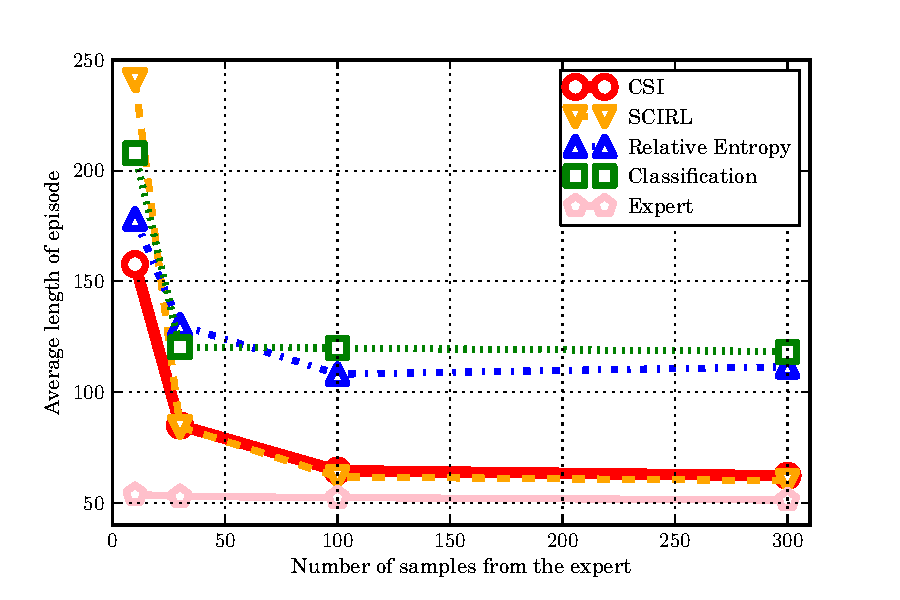
\includegraphics[width=\textwidth]{Exp11.pdf}
  \caption{Performance of various policies on the mountain car problem. This is the mean over 50 runs.}
  \label{fig:MountainCar}
\end{figure}

The classifier for CSI was an off-the-shelf SVM\footnote{\url{http://scikit-learn.org/stable/modules/generated/sklearn.svm.SVC.html}}, the regressor was an off-the-shelf SVR\footnote{\url{http://scikit-learn.org/stable/modules/generated/sklearn.svm.SVR.html}}.

\subsection{Highway driving simulator}
\label{subsec:highway}
The setting of the experiment is a driving simulator inspired from a benchmark already used in \cite{syed2008apprenticeship,syed2008game}. The agent controls a car that can switch between the three lanes of the road, go off-road on either side and modulate between three speed levels. At all timesteps, there will be one car in one of the three lanes. Even at the lowest speed, the player's car moves faster than the others. When the other car disappears at the bottom of the screen, another one appears at the top in a randomly chosen lane. It takes two transitions to completely change lanes, as the player can move left or right for half a lane's length at a time. At the highest speed setting, if the other car appears in the lane the player is in, it is not possible to avoid the collision. The main difference between the original benchmark \cite{syed2008apprenticeship,syed2008game} and ours is that we made the problem more ergodic by allowing the player to change speed whenever he wishes so, not just during the first transition. If anything, by adding two actions, we enlarged the state-action space and thus made the problem tougher.
%FIXME:METTRE UNE CAPTURE DECRAN.
The reward function $R_E$ the expert is trained by a DP algorithm on makes it go as fast as possible (high reward) while avoiding collisions (harshly penalised) and avoiding going off-road (moderately penalised). Any other situation receives a null reward.

%% The feature function $\phi$ for this setting is the natural tabular feature function where each state action couple $(s,a)$ is associated with a unique index $i_{(s,a)}$. The only non-zero component of $\phi(s,a)$ is then the component at index $i_{(s,a)}$.

The performance criterion for a policy $\pi$ is the mean (over the uniform distribution) value function with respect to $R_E$ : $\mathbf{E}_{s\sim\mathcal{U}}[V^{\pi}_{R_E}(s)]$. 

Expert performance averages to $7.74$ ; we also show the natural random baseline that consists in drawing a random reward vector (with a uniform law) and training an agent on it. The reward functions found by SCIRL, CSI and RE are then optimized using a DP algorithm. The dataset $D_{random}$ needed by RE (and neither by CSI nor SCIRL) is made of $100$ episodes of length $10$ starting randomly in the state space and following a random policy. the dataset $D_E$ is made of $n$ episodes of length $n$, with $n \in \{3,7,10,15,20\}$.


Results are shown Fig.~\ref{fig:Highway} and Tab.~\ref{tab:highway}. We give the values of $\mathbf{E}_{s\sim\mathcal{U}}[V^{\pi}_{R_E}(s)]$ with $\pi$ being in turn the optimal policy for the rewards given by SCIRL, CSI and RE, the policy $\pi_C$ of the classifier (the very one the classification step of CSI outputs), and the optimal policy for a randomly drawn reward. Performance for CSI is slightly but definitively higher than for SCIRL (see the variance in Tab.~\ref{tab:highway}), slightly below the performance of the expert itself. Very few samples (100) are needed to reliably achieve expert-level performance.

It is very interesting to compare our algorithm to the behavior of a classifier alone (respectively red and green plots on Fig.~\ref{tutu}). With \emph{the exact same data}, albeit the use of a very simple heuristics, the cascading approach demonstrates far better performance from the start. This is a clear illustration of the fact that using the Bellman equation to construct the data fed to the regressor and outputting not a policy, but a reward function that can be optimized on the MDP truly makes use of the information that the transitions $(s,a,s')$ bear (we recall that the classifier only uses $(s,a)$ couples).

Furthermore, the classifier whose results are diplayed here is the output of the first step of the algorithm. The classification performance is obviously not that good, this hints to the fact that our algorithm may be empirically more forgiving of classification errors than our theoretical bound lets us expect.
\begin{figure}
      \begin{tabular}{|l|l|l|l|l|}
        \hline
        &\bf CSI& \bf SCIRL& \bf RE& \bf Classif\\
        \hline \multicolumn{5}{|c|}{$n = 9$}\\ \hline
        Var& 5.139& 5.684& 4.686& 0.045 \\
        Min& -2.708& -3.175& -2.717& -1.564 \\
        Mean& 2.419& 2.762& 2.286& -1.149 \\
        Max& 7.050& 7.060& 7.027& -0.596 \\
        \hline \multicolumn{5}{|c|}{$n = 49$}\\ \hline
        Var& 0.214& 0.517& 0.701& 0.121 \\
        Min& 5.406& 4.652& 4.214& -1.148 \\
        Mean& 7.012& 6.784& 6.314& -0.158 \\
        Max& 7.454& 7.529& 7.465& 0.619 \\
        \hline \multicolumn{5}{|c|}{$n = 100$}\\ \hline
        Var& 0.011& 0.269& 0.486& 0.154 \\
        Min& 7.078& 5.724& 5.487& -0.574 \\
        Mean& 7.364& 7.194& 6.778& 0.456 \\
        Max& 7.526& 7.562& 7.509& 1.483 \\ \hline
        \end{tabular}
      \begin{tabular}{|l|l|l|l|l|}
        \hline
        &\bf CSI& \bf SCIRL& \bf RE& \bf Classif\\
        \hline \multicolumn{5}{|c|}{$n = 225$}\\ \hline
        Var& 0.006& 0.029& 0.146& 0.167 \\
        Min& 7.172& 5.882& 5.612& 0.128 \\
        Mean& 7.459& 7.377& 7.215& 1.151 \\
        Max& 7.563& 7.572& 7.578& 2.220 \\
        \hline \multicolumn{5}{|c|}{$n = 400$}\\ \hline
        Var& 0.002& 0.002& 0.005& 0.267 \\
        Min& 7.321& 7.247& 7.144& 0.041 \\
        Mean& 7.495& 7.369& 7.279& 1.744 \\
        Max& 7.552& 7.557& 7.519& 2.761 \\
        \hline
      \end{tabular}
      \caption{Raw results on the Highway driving problem, see how the variance of SCIRL and CSI decreases.}
     \label{tab:highway}
      \end{figure}
  \begin{figure}
   \subfigure[Mean performance over 100 runs on the Highway driving problem.]{\label{tutu}\includegraphics[width=.5\linewidth]{"Exp14"}}
   \subfigure[Zoom of Fig~\ref{tutu} showing the ranking of the three IRL algorithms.]{\includegraphics[width=.5\linewidth]{"Exp14_zoom"}}
  \caption{Results on the highway driving problem.}
  \label{fig:Highway}
  
\end{figure}


\section{Related Work}
\label{sec:related}
IRL was first introduced in \cite{russell1998learning} and then formalized in \cite{ng2000algorithms}. Approaches summarized in \cite{neu2009training} can be seen as iteratively contructing a reward function, solving an MDP at each iteration. Some of these algorithms are IRL algorithms while others fall in the Apprenticeship Learning (AL) category, as for example the projection version of the algorithm in \cite{abbeel2004apprenticeship}. In both cases the need to solve an MDP at each step may be very demanding, both sample-wise and computationally. CSI being able to output a reward function without having to solve the MDP is thus a significant improvement.

AL via classification has been proposed for example in \cite{ratliff2007imitation}, with the help of a structured margin method. Using the non trivial notion of metric in an MDP, the authors of \cite{melo2010learning} build a kernel which is used
in a classification algorithm, showing improvements compared to a
non-structured kernel.

Classification and IRL have met in the past in \cite{ratliff2006maximum}, but the labels were complete optimal policies rather than actions and the inputs were MDPs, which had to be solved. It may be unclear how SCIRL \cite{klein2012scirl} relates to the proposed approach of his paper. Both algorithms use the score function of a classifier as a proxy to the action-value function of the expert with respect to the (unknown) true reward: $Q^{\pi_E}_R$. The way this proxy is constructed and used, however, fundamentally differs in the two algorithms. This difference will cause the theoretical analysis of both approaches (see Sec.~\ref{sec:analysis}) to be distinct. In SCIRL, the score function of the classifier is approximated {\it via} a linear parametrization that relies on the feature expectation of the expert $\mu^E(s) = E[\sum_{t\geq 0}\gamma^t\phi(s_t)|s_0=s,\pi_E]$. This entails the use of a specific kind of classifier (namely linearly-parametrized-score-function-based classifiers) and of a method of approximation of $\mu^E$. By contrast, almost any off-the-shelf classifier can be used in the first step of the cascading approach of this paper. The classification step of CSI is unaware of the structure of the MDP whereas SCIRL knows about it thanks to the use of $\mu^E$. In CSI, the structure of the MDP is injected by reversing the Bellman equation prior to the regression step (Eq.~\ref{eq:rc} and \eqref{eq:rj}), a step that does not exist in SCIRL as SCIRL directly outputs the parameter vector found by its linearly-parametrized-score-function-based classifier. The regressor of CSI can be chosen off-the-shelf. One can argue that this and not having to approximate $\mu^E$ increases the ease-of-use of CSI over SCIRL and makes for a more versatile algorithm. In practice, as seen in Sec.~\ref{sec:experiments}, perfomance of SCIRL and CSI are very close to one another thus CSI may be a better choice as it is easier to deploy. We would like to emphasize the fact that although SCIRL and CSI share similarities, there exist key differences that we just explained. Neither approach is a generalization of the other.

Few IRL or AL algorithms do not require solving an MDP. The approach of \cite{syed2008apprenticeship} requires knowing the transition probabilities of the MDP (which CSI does not need) and outputs a policy (and not a reward). The algorithm in \cite{dvijotham2010inverse} only applies to linearly-solvable MDPs whereas our approach does not place such restrictions. Closer to our use-case is the idea presented in \cite{boularias2011relative} to use a subgradient ascent of a utility function based on the notion of relative entropy. Importance sampling is suggested as a way to avoid solving the MDP. This requires sampling trajectories according to a non-expert policy and
the direct problem remains at the core of the approach (even if
solving it is avoided).


\section{Conclusion}
\label{sec:conclusion}
We have introduced a new way to perform IRL by cascading two supervised approaches. The expert is theoretically shown to be near-optimal for the reward function the proposed algorithm outputs, given small classification and regression errors. Practical examples of classifiers and regressors have been given, and two combinations have been empirically (on two classic benchmarks) shown to be very resilient to dire lack of data on the input (only data from the expert was used to retrieve the reward function), provided the use of simple heuristics. On one of the benchmarks (a highway driving simulator), our algorithm is shown to outperform other state-of-the-art approaches. We plan on deepening the analysis of the theoretical properties of our approach and on applying it to real world robotics problems.

\bibliographystyle{plain}
\bibliography{Biblio}

\end{document}
